In order to profile the code that had been developed so far, the Oracle Developer Studio was used.
During testing, the code was run in serial with a single-rank and single-thread configuration.
For more obvious reductions in timings to be seen, the simulation was run with the following paramters:
$--L_x\quad 1\quad --L_y\quad 1\quad --N_x\quad 301\quad --N_y\quad 301\quad --T\quad 1\quad --dt\quad 0.005\quad --Re\quad 2000$.

The results from the profiling task are shown below in \tabl\ref{tab:optimise}. From running the serial code, it wwas noted that the main time spent was within the ``Solve'' method on the SCG class, as seen by \fig\ref{fig:time}.
\begin{figure}[H]
    \centering
        \centering
        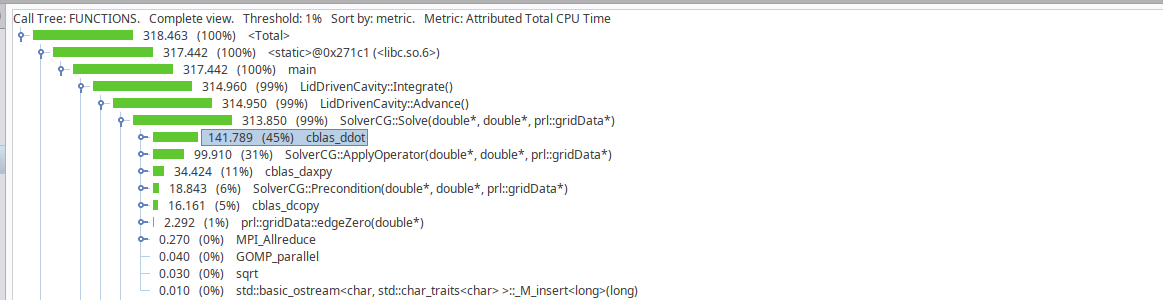
\includegraphics[height=4cm,width=\linewidth]{Images/time.png}
        \caption{Showing of which functions program spends most time in}
        \label{fig:time}

\end{figure}
\vspace*{-0.75cm}
Looking further it could be seen that through the useof BLAS the 2nd nested for loop could be removed from both the ``Precondition'' and ``ApplyOperator'' method.
From \tabl\ref{tab:optimise}, it can be seen that the changes implemented in the afformentioned methods, shown in \code\ref{lst:SCG}, resulted in reductions in function (inclusive) time of 42\% and 74\% respectively.
This was acheived htrough a stregic use of ``DAXPY'' and ``DSCAL'' methods. This approach was used beacuse the program can now compute the entire row needed in these methods as opposed to iterating through the entire grid and reevaluating the same values multiple times.
\begin{table}[H]
    \centering
        \caption{Shows changes to methods and reduction in timings, evidenced by \fig\ref{fig:optim}}
        \label{tab:optimise}
        \small
        \begin{tabular}{c|ccccc}
        \hline
        \textit{\textbf{Function}} & \textit{\textbf{Change}}                                                                                           & \textit{\textbf{\begin{tabular}[c]{@{}c@{}}Total \\ (Inclusive-CPU) \\ Time before\end{tabular}}} & \textit{\textbf{\begin{tabular}[c]{@{}c@{}}Total \\ (Inclusive-CPU) \\ Time after\end{tabular}}} & \textit{\textbf{\begin{tabular}[c]{@{}c@{}}Function \\ (Inclusive) \\ Time before\end{tabular}}} & \textit{\textbf{\begin{tabular}[c]{@{}c@{}}Function \\ (Inclusive) \\ Time after\end{tabular}}} \\ \hline
        ApplyOperator              & \begin{tabular}[c]{@{}c@{}}Replaced \\ interior nested\\ for loop with cblas\end{tabular}                          & 26.699                                                                                            & 21.395                                                                                           & 11.858                                                                                           & 6.825                                                                                           \\
        Precondition               & \begin{tabular}[c]{@{}c@{}}Replaced\\  interior nested\\ for loop with cblas\end{tabular}                          & 25.208                                                                                            & 21.355                                                                                           & 5.214                                                                                            & 1.381                                                                                           \\
        Advance                    & \begin{tabular}[c]{@{}c@{}}Replaced \\ interior nested\\ for loop with cblas \\ for current vorticity\end{tabular} & 41.079                                                                                            & 40.008                                                                                           & 39.598                                                                                           & 38.777                                                                                          \\
        Advance                    & \begin{tabular}[c]{@{}c@{}}Replaced\\  interior nested\\  for loop with cblas \\ to advance voritcity\end{tabular} & 40.028                                                                                            & 40.789                                                                                           & 38.677                                                                                           & 39.948                                                                                          \\ \hline
        All Changes                & \begin{tabular}[c]{@{}c@{}}Implemented \\ changes \\ above \\ compared \\ to none\end{tabular}                     & 456.83                                                                                            & 317.892                                                                                          & -                                                                                                & -                                                                                               \\ \hline
        \end{tabular}
        \end{table}
On the other hand when the same approach was taken within the LDC class, the results were not as expect. In the best case, the reduction in function time was 2\% and at worst caused an increase in function time of 3\%.
This can be noted due to the complexity of the algorithm needed to match the logic of the previous code. In order to evaluate the scheme which advances vorticity, over 12 lines of BLAS function calls had to be made to match this, as shown in \code\ref{lst:LDC}.
In the future if the simulation was run on a larger domain problem then a more modest result could be expected.

Overall, once the simulation had been run again with one MPI rank and one OPen MP thread but at larger time tomain, the performance improvements from profiling were clear.
All the changes when implemented compared to the base case after having just implemented Open MP, led to a reduction in overall inclusive CPU time of 30\%.